\chapter{Introduction}
\section{Repository Links}
\begin{itemize}
    \item VertexChat (Full Project Repository): \url{https://github.com/VertexChat}
	\item Vertex (Front-End User Interface): \url{https://github.com/VertexChat/vertex}
	\item Vertex (WebRTC Signalling Server): \url{https://github.com/VertexChat/webrtc-signalling-server}
	\item Norton (Back-End Server): \url{https://github.com/VertexChat/norton}
	\item Norton (API Client): \url{https://github.com/VertexChat/norton-api-client}
	\item Database: \url{https://github.com/VertexChat/database}
	\item Dissertation: \url{https://github.com/VertexChat/dissertation}
\end{itemize}
\section{Project Introduction}
The purpose of this project was to construct an application which relied on modern day frameworks and technologies. We aimed to use these technologies and frameworks to build a self-hosted conference application in which the user could generate their own sessions and chat rooms in order to communicate with others. We had intended to combine these technologies with pre-existing technologies such as WebRTC, or VOIP, to allow the success of the application. During the initial planning stage of this application we had no idea that the relevance of this application would become quite large and necessary due to the outbreak of COVID-19 and a solid conference call application would become heavy relied on for day-to-day work.
\\\\ The aim of this project was to combine a state-of-the-art front-end framework to a reliable and rapid back-end technology which would be connected to a stable and resilient database. The choices we examined and undertook were the following: Flutter, for the front-end; Flask, for the back-end; MySQL, for the database. A large aim for this project was also to integrate Flutter with WebRTC, which was quite a challenge as Flutter is still quite new and there exist few examples of the correct structure to which the challenge had presented.
\\\\ The result of this found that Flutter was perhaps not the best approach for this. Although it can be done, it was quite a laborious tool for the job and required quite a lot of skill which was quite difficult to obtain given the time-frame and nature of this project. Flask was proven to be reliable and easy to use, but the combination of Flutter alongside Flask posed the same cumbersome issues to which the WebRTC had given. This made for a tedious project with very little satisfactory output. 
\begin{figure}[h!]
    \caption{Application Icon}
    \label{image:vertexChatLogo}
    \centering
    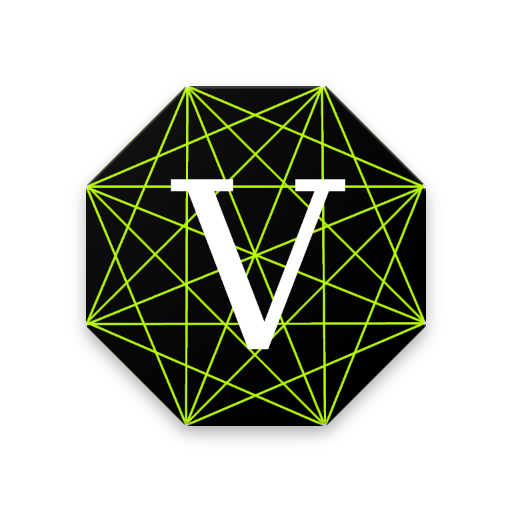
\includegraphics[width=0.8\textwidth]{images/vertexChatLogo.png}
\end{figure}